%%
%% This is file `husttrans-example.tex',
%% generated with the docstrip utility.
%%
%% The original source files were:
%%
%% husttrans.dtx  (with options: `example')
%% 
%% This is a generated file.
%% 
%% Copyright (C) 2013-2014 by Xu Cheng <xucheng@me.com>
%%               2014-2016 by hust-latex <https://github.com/hust-latex>
%% 
%% This work may be distributed and/or modified under the
%% conditions of the LaTeX Project Public License, either version 1.3
%% of this license or (at your option) any later version.
%% The latest version of this license is in
%%   http://www.latex-project.org/lppl.txt
%% and version 1.3 or later is part of all distributions of LaTeX
%% version 2005/12/01 or later.
%% 
%% This work has the LPPL maintenance status `maintained'.
%% 
%% The Current Maintainer of this work is hust-latex Organization.
%% 
%% This work consists of the files husttrans.dtx,
%% husttrans.ins and the derived file husttrans.cls
%% along with its document and example files.
%% 
%% \CharacterTable
%% {Upper-case    \A\B\C\D\E\F\G\H\I\J\K\L\M\N\O\P\Q\R\S\T\U\V\W\X\Y\Z
%%  Lower-case    \a\b\c\d\e\f\g\h\i\j\k\l\m\n\o\p\q\r\s\t\u\v\w\x\y\z
%%  Digits        \0\1\2\3\4\5\6\7\8\9
%%  Exclamation   \!     Double quote  \"     Hash (number) \#
%%  Dollar        \$     Percent       \%     Ampersand     \&
%%  Acute accent  \'     Left paren    \(     Right paren   \)
%%  Asterisk      \*     Plus          \+     Comma         \,
%%  Minus         \-     Point         \.     Solidus       \/
%%  Colon         \:     Semicolon     \;     Less than     \<
%%  Equals        \=     Greater than  \>     Question mark \?
%%  Commercial at \@     Left bracket  \[     Backslash     \\
%%  Right bracket \]     Circumflex    \^     Underscore    \_
%%  Grave accent  \`     Left brace    \{     Vertical bar  \|
%%  Right brace   \}     Tilde         \~}

\documentclass{husttrans}
\usepackage{multicol}

\title{电子通信系统的原理}
\author{路易斯·F·弗伦泽尔}
\translator{祁雨霏}
\supervisor{黑晓军\hspace{1em}副教授}
\date{2014}{3}{1}

\begin{document}

\frontmatter
\maketitle
\tableofcontents
\mainmatter
\chapter{传输线}
通信中的传输线路传送电话信号,局域网中的计算机数据,有线电视系统中的电视和互联网信号以及信号
从发射机到天线或从天线到接收机。传输线也是连接设备的短电缆或将嵌入式微计算机连接到其他设备的印刷电路板铜线
电路通过各种接口的方式。 传输线是关键链接任何通讯系统。 它们不仅仅是电线或电缆。他们的电气特性是至关重要的,必须与之匹配成功的沟通发生的设备。

\begin{description}\Large
\item\hei{目标}
\end{description}
\vskip\baselineskip
完成本章后,您将能够:
\begin{itemize}
\item 命名不同类型的传输线并列出每个传输线的具体应用。
\item 说明传输线可以用作调谐电路和电抗元件的情况。
\item 定义特征阻抗并通过几种不同的方法计算传输线的特征阻抗。
\item 计算波长的传输线长度。
\item 定义驻波比(SWR),解释其对传输线设计的意义,并用阻抗值或反射系数计算SWR。
\item 陈述完美匹配线的标准,并描述产生不适当匹配线的条件。
\item 使用史密斯圆图进行传输线计算。
\item 定义带状线和微带,并说明它们在哪里以及如何使用。
\end{itemize}

\section{传输线基础}\label{sec:1}
传输线的两个主要要求是(1)线路对信号引入最小的衰减,(2)线路不将任何信号作为无线电能量辐射。 所有的传输线和连接器都是根据这些要求而设计的。\marginpar[10pt]{传输线}
\subsection{传输线的类型}
\subsubsection{并行线路}
平行线路由两个平行的导体制成,两个平行的导体由1/2英寸到几英寸的间隔隔开。 图13-1(a)显示了一个双线平衡线,其中使用绝缘垫片来保持导线分离。 这种线如今很少使用。 平行线的变化是图13-1(b)所示的300V双引线类型,其中线之间的间距由连续塑料绝缘体保持。并行线如今很少使用。\marginpar{平行线路}
\subsubsection{同轴电缆}
传输线使用最广泛的类型是同轴电缆,它由一个绝缘材料包围的实心中心导体组成,通常是一个塑料绝缘体,如Tel [见图13-1(c)]。 也可以使用空气或气体电介质,其中中心导体通过周期性绝缘间隔保持就位。 绝缘体上方是第二根导线,管状编织物或由电线组成的屏蔽层。 外部塑料护套保护和隔离编织物。 同轴电缆有多种尺寸,直径从大约1/4英寸到几英寸。\marginpar{同轴电缆}
\subsubsection{双绞线}
正如其名称所示,双绞线电缆使用两根绝缘并被松散地绞合在一起的绝缘实心铜线。 参见图13-1(d)。 这种电缆原来是用在电话线路上的,现在还在使用,但也用于传感器和其他设备的安全系统接线。 并且双绞线,就像你在Chap看到的那样。 12是局域网(LAN)中使用最广泛的布线类型之一。 它通常被称为非屏蔽双绞线(UTP)电缆。 处理低频音频或高频脉冲的电缆有多种等级。 电线的尺寸,绝缘的类型和捻度(每英捻)的紧密性决定了它的特性。 它有一个整体编织屏蔽,被称为屏蔽双绞线(STP)电缆。 最常见的版本包含在一个共同的绝缘油管内的四对。
\marginpar{同轴电缆的主要优点是完全屏蔽,因此外部噪声几乎没有影响。}
\bigskip
\hrule
\medskip
\noindent\textbf{图13-1}传输线路的常见类型 (a)露天电话线。 (b)开放式电线称为300V双引线。 (c)同轴电缆(d)双绞线。\\
\begin{figure}[!h]
\centering
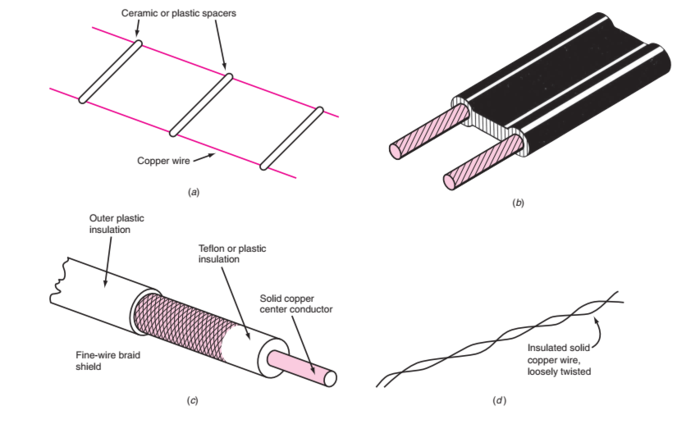
\includegraphics[width=.8\textwidth]{01.png}
\end{figure}

\subsection{平衡线与非平衡线}
传输线可以平衡或不平衡。 一条平衡线是没有线连接到地面的线。 相反,每条线上的信号都是以地为参考的。 尽管一根导线中的电流方向与另一根导线中的电流相差180°,但每根导线中的电流相对于地线都相同。在不平衡的线路中,一个导体接地。 双绞线[图13-1(d)]可用于平衡或不平衡的安排,但平衡形式更为常见。\\
\indent 开放的线路有一个平衡的配置。 图13-2(a)显示了一个典型的馈电装置。 驱动发生器和接收电路是中心抽头变压器,其中中心抽头接地。 均衡的电线提供显着的保护,防止噪音和串音。 由于平衡线路上信号的极性相同,任何引入电缆的外部信号同时出现在两条线路上,但是在接收器处被抵消。 这就是所谓的共模抑制,降噪可以高达60到70分贝。\\
\indent 图13-2(b)显示了一条不平衡线路。 同轴电缆是不平衡的线路; 中心导体中的电流以连接到地面的编织物为参考。同轴电缆和屏蔽双绞线电缆对由于外部信号引起的电感或电容耦合的噪声拾取或串扰提供了明显但不完全的保护。 未屏蔽的线路可能会拾取信号和串音,甚至可能辐射能量,导致不希望的信号丢失。\\
\indent 有时需要或希望将平衡转换为不平衡操作,反之亦然。 这是通过一个称为平衡 - 不平衡转换器的设备完成的。\\
\bigskip
\hrule
\medskip
\noindent\textbf{图13-2}(a)平衡线。 (b)不平衡线路。\\
\begin{figure}[!h]
\centering
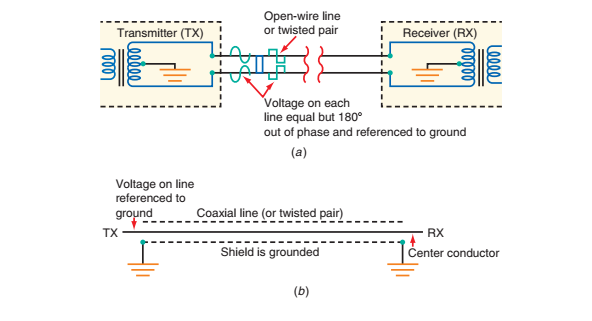
\includegraphics[width=.8\textwidth]{02.png}
\end{figure}

\subsection{电缆波长}
将60Hz电力线信号传输到家中的双线电缆是传输线,将立体声接收器的音频输出连接到立体声扬声器的电线也是如此。在这些低频下,传输线充当交流电压的载波。 对于这些应用,感兴趣电缆的唯一特征是电阻损耗。 低频线路的尺寸和电气特性可以有很大的不同,而不会影响性能。导体尺寸是一个例外,它决定了长距离的电流承载能力和电压降。 导体的电气长度通常比它们携带的频率的1个波长短。除非在信号频率上至少0.1λ长,否则一对载流导体不被认为是传输线。\\
\indent 用来携带射频能量的电缆不是简单的电阻导体,而是电感,电容和电阻的复杂等价物。 此外,每当传输线的长度与传输信号的波长相同或更大时,该线具有特殊的特性并需要更复杂的分析。\\
\indent 如前所述,波长是交流波的一个周期的长度或距离或交流波在该信号的一个周期所需的时间内行进的距离。 在数学上,波长λ是光速与信号频率f之比:λ=300,000,000/f,其中3亿是光速,以米/秒为单位,在自由空间或空气中(300,000,000m/s < 186,400mi/秒),f的单位是赫兹。这也是无线电信号的速度。\\
\indent 那么60赫兹电力线信号的波长就是这样
$$\lambda = \frac{300,000,000}{60} = 5×10^6m$$
这是一个令人难以置信的长距离——数千英里。这种频率的实际传输线路距离当然要小得多。 然而,在无线电频率上,说3MHz或更多,波长变得相当短。3MHz的波长λ = 300,000,000 / 3,000,000 = 100m,距离300英尺多一点,或足球场的长度。这是一个非常实用的距离。随着频率变高,波长变短。在较高的频率下,波长公式简化为λ= 300/f,频率以兆赫为单位。50-MHz信号的波长为6m。通过使用脚而不是米,波长公式变为λ= 984/f,其中f以兆赫(λ现在以英尺表示)。\\
\indent 如果波长是已知的,频率可以计算如下:
$$f(MHz) = \frac{300}{\lambda(m)} \qquad or \qquad f(MHz) = \frac{984}{\lambda(ft)}$$\\
\indent 由给定电缆中的波长表示的距离取决于电缆的类型。 电缆中的速度可以是空间中光波(无线电波)速度的0.5至0.95倍,并且电缆中的信号波长将按比例小于空间中的信号波长。 因此,计算的电缆长度比自由空间中的波长短。 这在后面讨论。
\bigskip
\hrule
\medskip
\noindent\textbf 例13-1\\
\noindent 对于450MHz的工作频率,一对导体的长度被认为是一条传输线? (一对导体除非长度至少为0.1λ,否则不能用作传输线。)\\
$$λ = \frac{984}{450} = 2.19ft$$
$$0.1 λ = 2.19(0.1) = 0.219 ft (2.628 in)$$

\bigskip
\hrule
\medskip
\noindent\textbf 例13-2\\
\noindent 计算例13-1中传输线的物理长度a 3/8λ长。\\
$$\frac{3}{8}λ = \frac{2.19(3)}{8} = 0.82 ft (9.84 in)$$

\subsection{连接器}
大多数传输线终止于某种连接器,一种将电缆连接到设备或另一根电缆的设备。 普通的交流电源插头和插座是基本的连接器类型。 平行线和同轴电缆使用特殊连接器。 通信设备中无处不在的连接器通常被认为是理所当然的。 这是不幸的,因为它们在许多应用中是常见的故障点。
\subsubsection{同轴电缆连接器}
同轴电缆需要特殊的连接器,以保持电缆的特性。 尽管内部导体和屏蔽编织层在理论上可以用螺钉作为平行线来固定,但结果将是电气属性的剧烈变化,导致信号衰减,失真和其他问题。 因此,同轴连接器不仅设计为提供连接和断开设备和电缆的便利方式,而且还保持电缆的物理完整性和电气特性。\\
\indent 同轴连接器的选择取决于电缆的类型和尺寸,操作频率以及应用。 最常见的类型是PL-259或UHF,BNC,F,SMA和N型连接器。\\
\indent PL-259连接器如图13-3(a)所示。 PL-259的内部结构和连接原理如图13-3(b)所示。 连接器的主体被设计成围绕同轴电缆的末端,并提供方便的方法来连接屏蔽编织层和内导体。 内导体被焊接到一个公接脚,该公接脚与连接器的主体绝缘,焊接或压接到编织物上。 一个耦合器在身体上; 它具有内螺纹,允许连接器连接到名为SO-239的母连接器上的匹配螺纹。 参见图13-3c。\\
\indent PL-259也被称为UHF连接器,虽然在HF和VHF上使用得更广泛,但可用于最低UHF值(小于500 MHz)。 它可以同时容纳大型(高达0.5英寸)和小型(0.25英寸)的同轴电缆。\\
\indent 另一个非常受欢迎的连接器是BNC连接器(图13-4)。 BNC连接器广泛用于0.25英寸的同轴电缆,用于将测试仪器(如示波器,频率计数器和频谱分析仪)连接到被测设备上。 BNC连接器也广泛用于局域网和一些UHF无线电的0.25英寸同轴电缆。\\
\indent 在BNC连接器中,电缆的中心导体焊接或压接到公针上,屏蔽层连接到连接器的主体上。 外壳或耦合器旋转,通过旋转耦合器上的销钉和凸轮通道将连接器物理连接到配套的母连接器[见图13-4(b)]。\\
\indent BNC连接器的众多变体之一是允许两根电缆首尾相连的圆筒形连接器和T型连接器,
(见图13-4(a)和(d)]。 另一个变体是SMA连接器,它使用螺纹而不是凸轮槽和销(图13-5)。 SMA连接器的特点是公连接器主体的六边形形状。 像BNC连接器一样,它使用较小的同轴电缆。\\

\bigskip
\hrule
\medskip
\noindent\textbf{图13-3} UHF连接器 (a)PL-259公连接器。(b)PL-259的内部结构和连接。(c)SO-239母型机箱连接器。\\
\begin{figure}[!h]
\centering
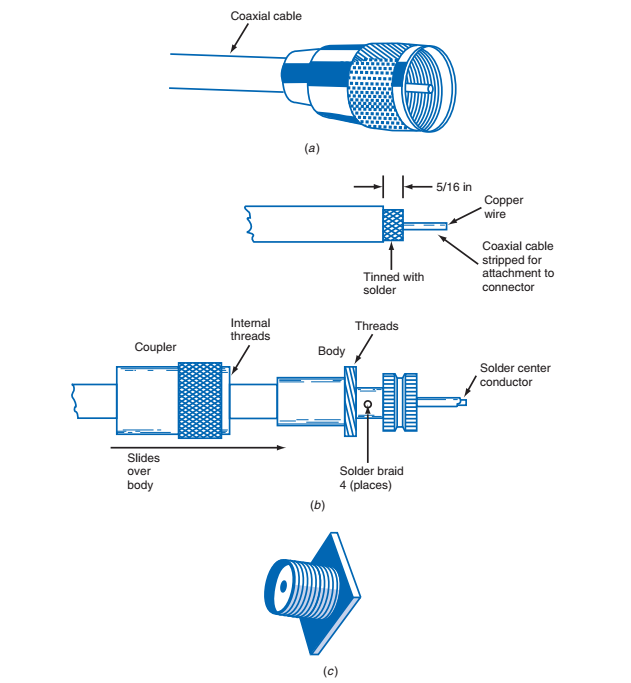
\includegraphics[width=.8\textwidth]{03.png}
\end{figure}
\bigskip
\bigskip
\bigskip

\bigskip
\hrule
\medskip
\noindent\textbf{图13-4} BNC连接器 (a)男士。(b)女性。(c)桶式连接器。(d)T型连接器。\\
\begin{figure}[!h]
\centering
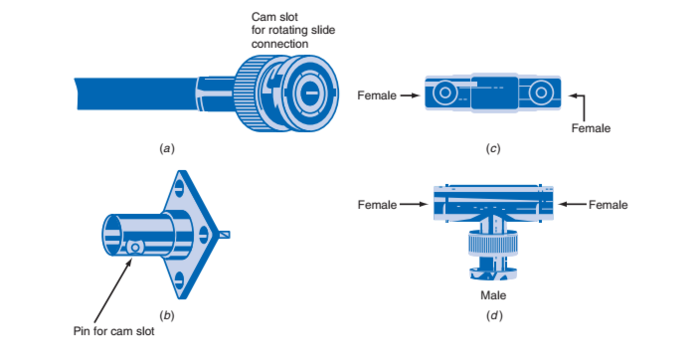
\includegraphics[width=.8\textwidth]{04.png}
\end{figure}
\bigskip
\bigskip
\bigskip

\bigskip
\hrule
\medskip
\noindent\textbf{图13-5} SMA连接器。\\
\begin{figure}[!h]
\centering

\includegraphics[width=.8\textwidth]{05.png}
\end{figure}

\indent 最便宜的同轴电缆连接器是F型连接器,广泛用于电视机,录像机,DVD播放机和有线电视。 电缆插头及其匹配的机箱插孔如图13-6所示。 同轴电缆的屏蔽被压接到连接器上,而电缆的实心导线中心导体而不是单独的引脚被用作连接。 将六角形外圈拧入以将插头连接到配对插孔。\\
\indent 另一种廉价的同轴连接器是众所周知的RCA留声机连接器(图13-7),主要用于音频设备。 这款多功能低成本设备最初是在60多年前设计的,用于将唱机拾音器从转盘连接到放大器,这些多功能和低成本的设备可用于无线电频率,并已用于低VHF范围的电视机连接。\\
\indent 性能最好的同轴连接器是N型连接器(图13-8),主要用于较高频率的大型同轴电缆,包括UHF和微波。 N型连接器是复杂且昂贵的,但是在维持通过互连的电缆的电特性方面比其他连接器做得更好。\\

\bigskip
\hrule
\medskip
\noindent\textbf{图13-6} F连接器用于电视机,录像机和有线电视盒。\\
\begin{figure}[!h]
\centering
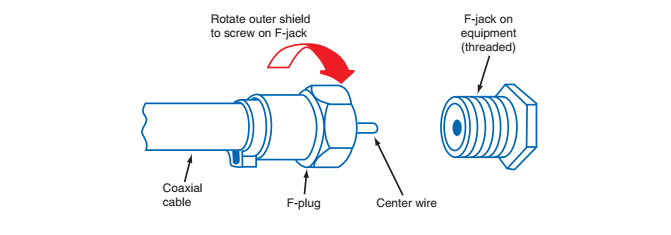
\includegraphics[width=.8\textwidth]{06.png}
\end{figure}

\bigskip
\hrule
\medskip
\noindent\textbf{图13-7} RCA留声机连接器有时用于直到VHF的射频连接器。\\
\begin{figure}[!h]
\centering
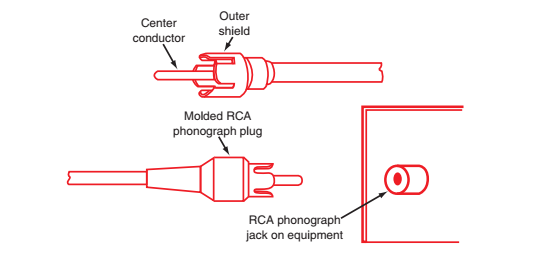
\includegraphics[width=.8\textwidth]{07.png}
\end{figure}

\bigskip
\hrule
\medskip
\noindent\textbf{图13-8} N型同轴连接器。\\
\begin{figure}[!h]
\centering

\includegraphics[width=.8\textwidth]{08.png}
\end{figure}

\subsection{特性阻抗}
当传输线的长度在信号频率上比几个波长长时,传输线的两个平行导体表现为复阻抗。 这些电线表现出相当大的串联电感,其电抗在高频率下显着。 与该电感串联的是导线或导线的编织物的电阻,其包括固有的欧姆电阻加上由趋肤效应引起的任何电阻。 此外,平行导体与绝缘体形成分布电容,绝缘体充当电介质。 另外,由于导体之间的绝缘缺陷,导致电缆两端有分路或漏电阻或电导(G)。 结果是,对于高频信号,传输线表现为由串联电感器和电阻器以及并联电容器和电阻器组成的分布式低通滤波器[图13-9(a)]。 这被称为分布式线路的集总模型。\\
\indent 在图13-9(b)中的简化等效电路中,电感,电阻和电容已经组合成较大的等效块。 分流漏电阻非常高,影响可以忽略不计,所以忽略不计。 在该线的短段中,导体的串联电阻有时可以被忽略,因为它太低而不能被忽略。 然而,在较长的长度上,这个电阻会造成相当大的信号衰减。 电感和电容的影响是相当大的,事实上它们决定了线路的特性。\\
\indent 连接到这种传输线的RF发生器看到的阻抗是电路中的电感,电阻和电容的函数 - 特性或浪涌阻抗$Z_0$。 如果我们假设线路的长度是无限的,那么这个阻抗是电阻的。 如果等于特性阻抗的阻性负载连接到线路的末端,则特性阻抗对于有限的线路也是纯阻性的。\\

\bigskip
\hrule
\medskip
\noindent\textbf{图13-9} 传输线表现为任何驱动发生器的分布式低通滤波器。 (a)具有集总组件的分布式线路。 (b)简化的等效电路。\\
\begin{figure}[!h]
\centering
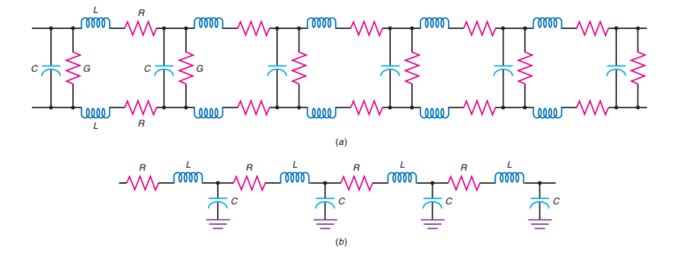
\includegraphics[width=.8\textwidth]{09.png}
\end{figure}

\bigskip
\hrule
\medskip
\noindent\textbf{图13-10} 负载电阻等于浪涌阻抗的传输线表现为与发生器等电阻。\\
\begin{figure}[!h]
\centering
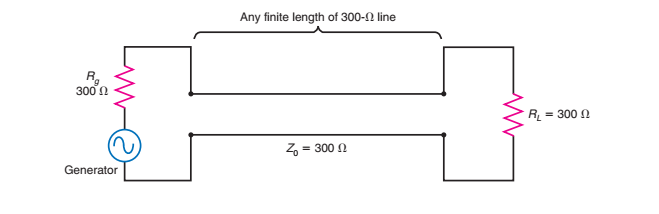
\includegraphics[width=.8\textwidth]{10.png}
\end{figure}


\subsubsection{由电感和电容确定$Z_0$}
对于一根长的传输线,特征阻抗$Z_0$由公式$Z_0 = \sqrt{L/C}$给出,其中$Z_0$是欧姆,L是给定长度的传输线的电感,C是相同长度的电容。 如果传输线终止于一个等于特征阻抗的负载电阻(见图13-10),那么该公式即使在有限的长度内也是有效的。 这是任何应用中传输线的正常连接。 在等式中,
$$R_L = Z_0$$\\
\indent 如果使线路,负载和发电机阻抗相等,匹配的发电机和负载电阻就是这样,满足最大功率传输的标准。\\
\indent 可以使用阻抗测量仪或电桥来测量一段平行线或同轴电缆的电感和电容,以获得计算阻抗所需的值。 假定,例如,测量100英尺的0.0022μF(2200pF)的电容,每个导体的电感被单独测量,然后相加,总共5.5μH。 (由于电阻没有进入特性阻抗的计算,所以忽略电阻,但会造成长距离的信号衰减)。那么浪涌阻抗是
$$Z_0 = \sqrt{\frac{L}{C}} = \sqrt{\frac{5.5×10^{-6}}{2200×10^{-12}}} = \sqrt{2500} = 50Ω$$
在实践中,没有必要进行这些计算,因为电缆制造商总是指定阻抗。\\
\indent 电缆的特性阻抗与长度无关。 我们通过使用L和C的值来计算100 ft,但50 V是1 ft或1000 ft的正确值。请注意,实际阻抗只有在电缆长度为几个波长或更多时才接近计算阻抗 终止于其特征阻抗。 对于小于1.0λ的线路长度,特性阻抗并不重要。\\
\indent 大多数传输线都带有标准的固有特性阻抗值。 例如,广泛使用的双引线平衡线[图13-1(b)]具有300V的特征阻抗。[图13-1(a)],这是不再广泛使用,是用450和600 V的阻抗。同轴电缆的共同特征阻抗是52,53.5,75,93和125 V。\\

\subsection{速度因子}
传输线应用中一个重要的考虑因素是传输线中的信号速度比自由空间中的信号速度慢。电缆中信号的传播速度小于自由空间中光传播速度的一个部分,称为速度因子(VF),它是传输线Vp的速度与自由速度的比值 空间Vc:
$$VF = \frac{V_p}{V_c} \qquad or \qquad VF = \frac{V_p}{c}$$
其中Vc = c = 300,000,000m/s\\
\indent 传输线中的速度因子从大约0.5到0.9变化。 同轴电缆的速度因数通常为0.6至0.8。 开路线的VF大约为0.9,而300-V双引线的速度因子大约为0.8。\\
\subsubsection{计算速度因子}
线路中的速度因子可以用表达式$VF = 1/ \sqrt{ε}$来计算,其中ε是绝缘材料的介电常数。例如,如果同轴电缆中的电介质是Tel,那么介电常数是2.1,速度因子 是$1/\sqrt{12.1} = 1/1.45 = 0.69$。 也就是说,同轴电缆中的信号速度是光速的0.69倍,即0.69×300,000,000=207,000,000m/s(128,616mi/s)\\
\indent 如果假定无损(零电阻)线,则可以用表达式计算传播速度的近似值
$$V_p = \frac{1}{\sqrt{LC}}\qquad ft/s$$
其中l是以英尺或其他长度单位表示的信号的行进长度或总距离,并且L和C以相同的单位给出。 假设例如具有50V的特征阻抗和30pF / ft的电容的同轴电缆。 每英尺的电感为0.075μH或75 nH。 在这根电缆每英尺的传播速度是
$$V_p = \frac{1}{\sqrt{75×10^{-9}×30×10^{-12}}} = 6.7×10^{8}ft/s$$
or 126,262mi/s,or $204×10^{6}$m/s\\
\indent 速度因子是
$$VF = \frac{V_p}{V_c} = \frac{204×10^{6}}{300×10^{6}} = 0.68$$\\
\subsubsection{计算传输线长度}
在计算波长的传输线长度时,必须考虑速度因子。 有时需要使用特定类型传输线的一半或四分之一波长用于特定的目的,例如阻抗匹配,滤波和调谐。\\
\indent 之前给出的自由空间中信号的一个波长的公式是λ = 984/f。 然而,这个表达式必须由速度因子来修正,以达到传输线的真实长度。 新的公式是
$$λ(ft)= 984\frac{VF}{f(MHz)}$$
假设,例如,我们想要找到在30MHz的VF为0.65的同轴电缆的四分之一波长段的实际长度(以英尺为单位)。 使用公式给出λ= 984(VF/f)= 984(0.65/30)= 21.32ft。以英尺为单位的长度是其的四分之一,即21.32/4 = 5.33ft。\\
\indent 用于计算给定传输线正确长度的正确速度因子可以从制造商的文献和各种手册中获得。\\


\bigskip
\hrule
\medskip
\noindent\textbf{图13-11} 传输线路延时对信号的影响 (a)正弦波延迟导致滞后相移。 (b)脉冲延迟。\\
\begin{figure}[!h]
\centering
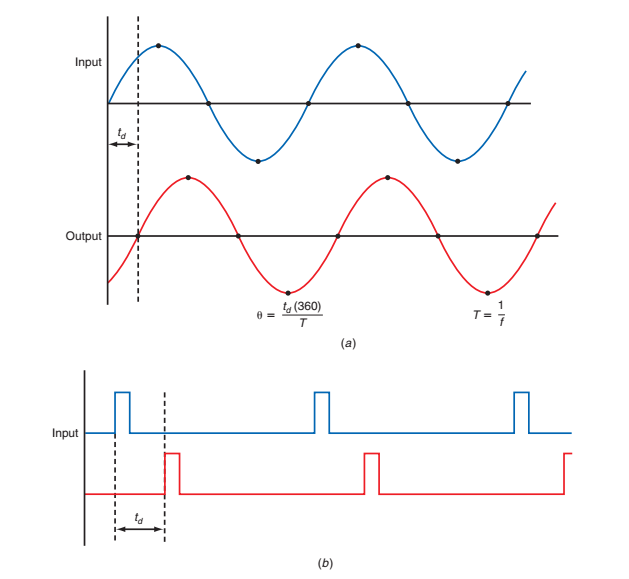
\includegraphics[width=.8\textwidth]{11.png}
\end{figure}


\subsection{时间延迟}
由于传输线的传播速度小于自由空间的传播速度,所以假定任何一条线都会减慢或延迟施加于其上的信号是合理的。 在一条线的一端施加的信号在一段时间之后出现在线的另一端。 这称为线路的时间延迟或传输时间。 为了实现延迟,特别使用的传输线称为延迟线。\\
\indent 图13-11显示了时间延迟对正弦波信号和脉冲串的影响。 输出的正弦波比输入时间更晚出现,所以它的相位发生了相移。 效果与通过电抗电路引入滞后相移相同。 在脉冲序列的情况下,脉冲延迟取决于延迟线的类型和长度。\\
\indent 延迟时间的长短是线路电感和电容的函数。 与由电感提供的电流变化以及电容的充电和放电时间的相反导致无限延迟。 这个延迟时间是用表达式计算的
$$t_d = \sqrt{LC}$$
其中td是以秒为单位的,L和C分别是线路单位长度的电感和电容。 如果L和C以英尺为单位给出,则延迟时间将是每英尺。例如,如果特定线路的电容为30pF / ft,电感为0.075μH/ ft,则延迟时间为
$$t_d = \sqrt{0.075×10^{-6}×30×10^{-12}} = 1.5×10^{-9}or1.5 ns/ft$$
这条50英尺长的线路将引入1.5 × 50 = 75ns的延迟。\\
\indent 同轴电缆引入的时延也可以用公式计算
$$t_d = 1.016\sqrt{ε}ns/ft$$
其中$t_d$是每英尺纳秒的时间延迟,ε是电缆的介电常数。\\
\indent 例如,由介电常数为2.3的75英尺电缆引入的总时间延迟是
$$t_d = 1.016\sqrt{ε} = 1.016\sqrt{2.3} = 1.016(1.517) = 1.54 ns/ft$$
总延迟时间为1.54(75)= 115.6 ns。\\
\indent 为了确定由延迟表示的相移,必须知道正弦波的频率和周期。 一个周期的周期或时间T可用众所周知的公式T = 1 /f来确定,其中f是正弦波的频率。假设频率为4MHz。 期间是
$$T = \frac{1}{4×10^{6}} = 250 × 10^{-9} = 250ns$$\\
\indent 先前描述的延迟75ns的50英尺线的相移由下式给出
$$θ= \frac{360t_d}{T} = \frac{360(75)}{250} = 108°$$\\
\indent 在射频应用中,传输线延迟通常被忽略,并且在无线电通信中实际上是不相关的。 但是,在时间很重要的高频应用中,传输线延迟可能是重要的。 例如,在局域网中,同轴电缆上二进制脉冲的转换时间往往是计算最大允许电缆长度的决定性因素。\\
\indent 某些应用需要精确的时间和信号的排序,特别是脉冲。 同轴延迟线可用于此目的。 很显然,大卷同轴电缆在现代电子设备中并不是一个方便的组件。 结果,人造延迟线已经被开发出来。 它们由作为低通滤波器连接的单个电感器和电容器组成,以模拟分布式传输线。或者,可以构造更紧凑的分布式延迟线,其由缠绕金属形式的绝缘线圈构成。 线圈提供分布电感,同时作为一个分布电容器的一个板。 金属形式是另一个板。 这种延迟线在电视机,示波器,雷达装置等电子设备中广泛使用。\\

\subsection{传输线规格}
图13-12总结了几种常用类型同轴电缆的规格。许多同轴电缆由字母RG或制造商的部件号开头的字母数字代码指定。主要规格是特性阻抗和衰减。其他重要参数是最大击穿电压额定值,每英尺电容,速度系数和外径(以英寸为单位)。衰减是每100英尺电缆损失的功率量,以100兆赫的分贝表示。衰减与电缆长度成正比,随频率增加。衰减与频率的详细图表也是可用的,以便用户可以预测其应用的损失。图13-13绘制了四种同轴电缆类型的衰减与频率的关系曲线。损失在非常高的频率是显着的。但是,电缆越大,损耗就越低。为了便于比较,请看图13-12中列出的300 V双引线电缆的特性。注意与同轴电缆相比损耗低。\\


\bigskip
\hrule
\medskip
\noindent\textbf{图13-12} 常用传输线特性表。\\
\begin{figure}[!h]
\centering
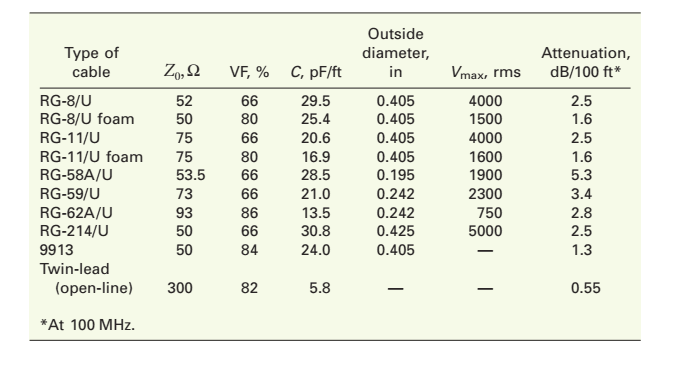
\includegraphics[width=.8\textwidth]{12.png}
\end{figure}

\bigskip
\hrule
\medskip
\noindent\textbf 例13-3\\
\noindent 正在使用100 MHz的RG-58A / U的165英尺部分将发射机连接到天线。 它在100MHz下100英尺的衰减是5.3dB。 其来自发射机的输入功率是100W。天线的总衰减和输出功率是多少?\\
$$电缆衰减 = \frac{5.3dB}{100ft} =  0.053 dB/ft$$
$$总衰减 = 0.053 × 165 = 8.745 dB or -8.745$$
$$dB = 10log\frac{P_in}{P_out} and  P_out = P_in(log^{-1}\frac{dB}{10})$$
$$P_out = 100(log^{-1}\frac{-8.745}{10}) = 100log^{-1}(-0.8745)$$
$$P_out = 100(0.1335) = 13.35 W$$

\indent 电缆中的损耗可能是重要的,特别是在较高的频率下。 在例13-3中,发射机将100W放入线路中,但在线路末端,输出功率(施加到天线的信号的电平)仅为13.35W。主要损耗为86.65W 在传输线中作为热量消散。\\
\indent 可以做几件事情来减少损失。 首先,应该尽一切努力找到一种缩短发射机和天线之间距离的方法。 如果这不可行,则可以使用更大的电缆。 对于例13-3中的应用,使用了RG-58A / U电缆。 这根电缆的特性阻抗为53.5V,所以任何附近的值都会令人满意。 一种可能性是RG-8 / U,阻抗为52 V,衰减量仅为2.5 dB / 100 ft。更好的选择是9913电缆,阻抗为50 V,衰减为1.3 dB / 100英尺。\\

\bigskip
\hrule
\medskip
\noindent \textbf{图13-13} 普通同轴电缆的衰减与频率的关系 请注意,图上的两个比例都是对数的。\\
\begin{figure}[!h]
\centering
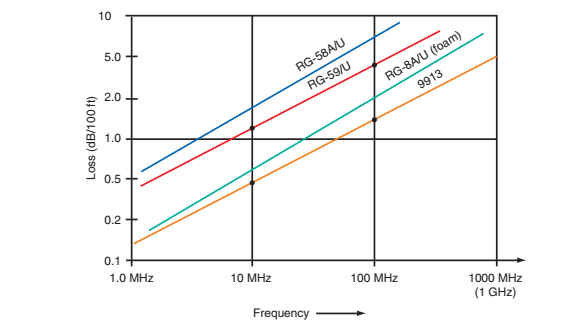
\includegraphics[width=.8\textwidth]{13.png}
\end{figure}

\indent 在考虑电缆长度和衰减之间的关系时,请记住,传输线是一个低通滤波器,其截止频率取决于线路和长度上的分布电感和电容。 线路越长,截止频率越低。 这意味着超过截止频率的更高频率的信号将以较快的速率下降。\\
\indent 这在图13-14中示出,其示出了四种常用类型的同轴电缆的衰减曲线。 请记住,截止频率是频率响应曲线上的3-dB下降点。 如果我们假设3 dB的衰减与3 dB的损耗相同,那么我们可以估计不同长度电缆的截止频率。 图中标出了3-dB的下降电平。 现在注意不同长度的电缆的截止频率。 较短的电缆(100英尺)具有最高的截止频率,带宽约为30 MHz。 200英尺电缆的截止频率约为8 MHz,500英尺电缆的截止频率约为2 MHz,而1000 ft电缆的截止频率约为1 MHz。 较高的频率通过,但由于电缆变长而严重衰减。 应该清楚,为什么使用较大的低损耗电缆,尽管成本较高,操作不方便,仍然需要更长时间的运行。\\
\indent 最后,增益天线可以用来抵消电缆损耗。 这些天线在第14章讨论。\\

\bigskip
\hrule
\medskip
\noindent\textbf{图13-14} RG-58A / U同轴电缆衰减与长度的关系 请注意,图上的两个比例都是对数的。\\
\begin{figure}[!h]
\centering
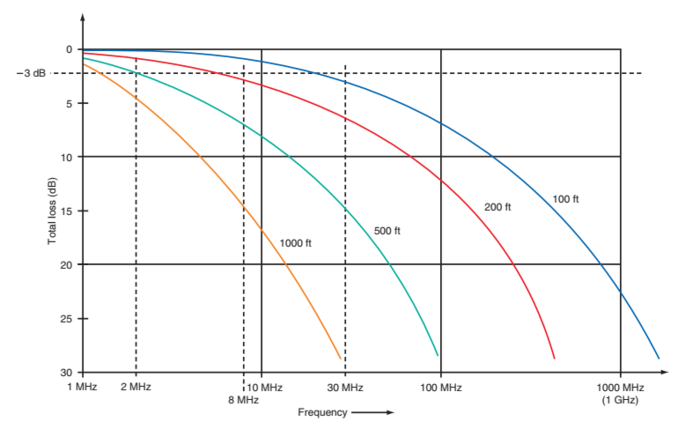
\includegraphics[width=.8\textwidth]{14.png}
\end{figure}

\bigskip
\hrule
\medskip
\noindent\textbf 例13-4\\
\noindent 一根长度为150英尺的RG-62A / U同轴电缆用作传输线。 找
(a)必须使用负载阻抗来终止线路以避免反向,
(b)每英尺的等效电感,(c)电缆引入的时间延迟,
(d)在2.5MHz正弦波上发生的相移,以及(e)以分贝为单位的总衰减。 (请参阅图13-12。)\\
\noindent a. 特性阻抗为93Ω; 因此负载必须提供93 V的电阻以避免反射。\\
\noindent b. $Z_0 = \frac{L}{C}$\quad $Z_0 = 93 Ω$\quad$C = 13.5 pF/ft$\quad
$L = CZ_0^{2}= 13.5 × 10^{-12} × (93)^{2} = 116.76 nH/ft$\\
\noindent $T = \frac{1}{f} = \frac{1}{2.5×10^{-6}} = 400ns$\quad
$θ = \frac{188.3(360)}{400} = 169.47°$\\
\noindent e. $Attenuation = \frac{2.8 dB}{100 ft} = 0.028 dB/ft$\quad
$150 ft × 0.028 dB/ft = 4.2 dB$\\


\section{驻波}
当一个信号被施加到传输线上时,由于传播延迟,它在一段时间之后出现在线的另一端。 如果在线路末端连接等于线路特性阻抗的阻性负载,则信号被负载吸收,功耗作为热量耗散。 如果负载是天线,则信号转换成电磁能并辐射到空间中。\\
\indent 如果线路末端的负载是开路或短路,或者线路的特性阻抗以外的阻抗,则信号没有被负载完全吸收。 当一条线路没有正确端接时,一些能量从线路的末端反射回来,并实际上回到线路上,朝向发电机。 这个相反的电压增加了正向或者发生的发电机电压,并且形成了一条沿着线路分布的复合电压。 这种电压模式及其相关电流构成了所谓的驻波。\\
\indent 驻波是不可取的。 反映表明发电机产生的功率没有被负载完全吸收。 在某些情况下,例如短路或开路,没有电力到达负载,因为所有的电力都被反馈到发电机。 以下各节将详细介绍如何生成驻波。\\

\subsection{反射与驻波之间的关系}
图13-15将用来说明如何产生相互作用以及它们如何促成驻波的形成。 (a)部分显示了直流脉冲如何沿着由相同LC部分组成的传输线传播。 电池(发电机)与开关一起用作输入信号以创建开/关直流脉冲。\\

\bigskip
\hrule
\medskip
\noindent\textbf{图13-15} 脉冲如何沿着传输线传播。\\
\begin{figure}[!h]
\centering
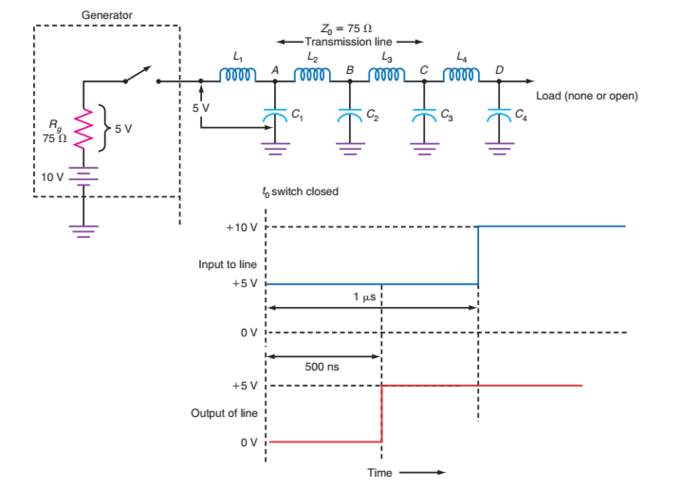
\includegraphics[width=.8\textwidth]{15.png}
\end{figure}

\indent 传输线在末端是开放的,而不是在线路的特征阻抗中终止。 一条开放的输电线路当然会产生反弹和驻波。 请注意,发生器的内部阻抗Rg等于传输线的特性阻抗。 假定传输线阻抗为75 V,内部发生器电阻为75 V.因此,由发生器提供的10 V在线路阻抗和内阻之间均匀分布。\\
\indent 现在假设开关闭合,将发电机连接到线路上。 如您所知,将直流电源连接到电感器和电容器等无功元件会产生瞬态信号,因为电感器会对抗电流变化,而电容器则会反抗电压变化。 当开关闭合时,电容器$C_1$最初起到短路的作用,但很快开始通过$L_1$向电池电压充电。 一旦A点的电压开始上升,它将对由$C_2$和$L_2$组成的传输线的下一部分施加一个电压。 因此,$C_2$开始通过$L_2$充电。 这个过程继续下去,直到$C_4$通过$L_4$充电,依此类推。 随着电容器充电,信号从左向右移动。 假定无损(零电阻)分量,并且最后电容器$C_4$最终充电到电源电压。\\
\indent 为了说明的目的,假设线路的长度和其他特性是这样的,延迟时间是500ns:在开关闭合500ns之后,输出脉冲将出现在线路的末端。 此时,输出电容$C_4$两端的电压等于5V或电源电压的一半。\\
\indent 输出电容充电至其最终值5V的瞬间,线路中的所有电流都停止,导致电感器周围的任何磁场崩溃。 存储在$L_4$的磁场中的能量等于存储在输出电容$C_4$中的能量。 因此,感应器中感应出5V的电压。 这个电压的极性将会增加到电容上已经存在的电荷的方向。这样,电容将充电到所施加的5V电压的两倍,即10V。\\
\indent 然后在L3中发生类似的效果。 $L_3$上的磁场崩溃,使$C_3$上的电压加倍。 接下来,$L_2$周围的磁场崩溃,将$C_2$充电至10 V。在$L_1$和$C_1$中出现相同的效果。 一旦信号到达线路的右端,电容器就会从右向左发生反向充电效应。 效果就好像一个信号从输出到输入一样。 从右向左移动的电荷是相对电流或相关波,发生器到输入端的输入波是入射波。\\
\indent 反射波需要500ns才能返回到发生器。 在1μs结束时,传输线的输入变为5V,总共为10V。\\
\indent 图13-15(b)显示了输入,输出和相对电压相对于时间的波形。 观察波形,按照前面描述的动作,在时间t0关闭开关。 由于线路的特性阻抗和内部发生器电阻均为75 V,因此电池电压的一半出现在点A的线路输入端。此电压沿线路传播,随线路电容器充电, 直到到达线的末端,并完全充电输出电容。 那时,电感中的电流开始停止,磁场崩溃,并且感应电压使线路末端的输出电压加倍。 因此在500ns之后,线路开路端的输出是10V。\\
\indent 相互作用开始,现在从右向左移动, 再过500ns后,它到达线路输入端,线路输入跳到10V。一旦停止反应,整个线路电容完全充电到10V,正如预期。\\
\indent 前面的描述涉及所谓的开路负载。 另一个极端的情况是短路负载。 对于这种情况,假设在图13-15(a)中跨$C_4$的短路。\\
\indent 当开关闭合时,再向输入端施加5V的电压,然后随着线电容器充电而沿线传播。因为线路的末端是短路的,所以电感器$L_4$实际上是该线路的负载。 $C_3$上的电压然后施加到$L_4$。此时,反射开始。 $L_4$中的电流崩溃,产生一个电压,然后沿着相反的方向向下传播。在$L_4$中感应的电压与沿线传播的电压相等而相反。因此,这个电压与$C_3$上的电压相等且相反,这导致$C_3$被放电。当接线从右向左进行时,线路电容会不断放电,直至到达发电机。电荷到达电线末端需要500 ns的时间,而相对于发电机则需要500 ns。因此,总共1μs时,输入电压从5V切换到0V。当然,输出短路两端的电压在整个时间内都保持为零。\\
\indent 开路和短路传输线有时被用来产生特殊效果。 然而,在实践中,传输线上的负载既不是零也不是0V; 相反,它通常是介于两者之间的某种价值。 负载可能是电阻性的,也可能有电抗性元件。天线通常没有完美的电阻值。 相反,他们经常有一个小的电容或电感电抗。 因此,负载阻抗相当于具有R ±jX形式的阻抗的串联RC或RL电路。 如果负载不完全是电阻性的并且等于线路的特性阻抗,则会产生相反的电压电平,具体取决于负载的复数阻抗。 通常一些功率被线路的电阻部分吸收; 不匹配仍会产生相反,但反射与原始信号不相等,如短路或开路负载的情况。\\
\indent 在大多数通信应用中,应用于传输线路的信号是交流信号。 假设信号是正弦波,可以分析这种情况。 该线对正弦波的影响类似于上面基于图13-15的分析的讨论中所描述的。 如果线路在与线路的特征阻抗相等的阻性负载中终止,则正弦波信号被负载完全吸收并且不发生反射。\\

\subsection{匹配线}
理想情况下,传输线应该在阻抗等于线路特性阻抗的负载中终结。 这被称为匹配线。 例如,如图13-16所示,50 V同轴电缆应采用50V电阻进行端接。 如果负载是天线,那么这个天线应该看起来像50V的电阻。当线路的负载阻抗和特性阻抗匹配时,传输平滑并且最大功率传输 - 线路中的任何电阻损耗 地点。 该行可以是任何长度。 设计天线和传输线系统的关键目标之一是确保这一匹配。\\

\bigskip
\hrule
\medskip
\noindent\textbf{图13-16} 传输线路的特性阻抗必须终止,才能正常工作。\\
\begin{figure}[!h]
\centering
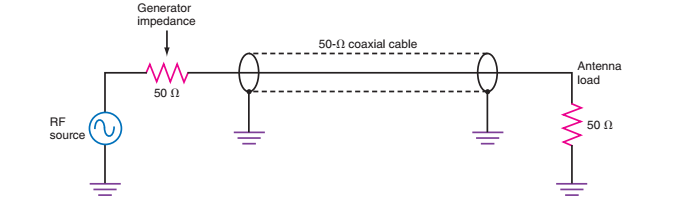
\includegraphics[width=.8\textwidth]{16.png}
\end{figure}

\indent 匹配线路上任何一点的交流电压(或电流)都是一个常数值(不考虑损耗)。 因此,正确端接的传输线被认为是平坦的。 例如,如果电压表从发生器到负载的匹配线下移,绘制有效值电压值,则波形对电压线的结果将为1(见图13-17)。 线路中的阻性损耗当然会沿着线路产生一个小的压降,使其向下倾斜的时间更长。\\


\bigskip
\hrule
\medskip
\noindent\textbf{图13-17} 匹配线上的电压在整个长度上是恒定的。\\
\begin{figure}[!h]
\centering
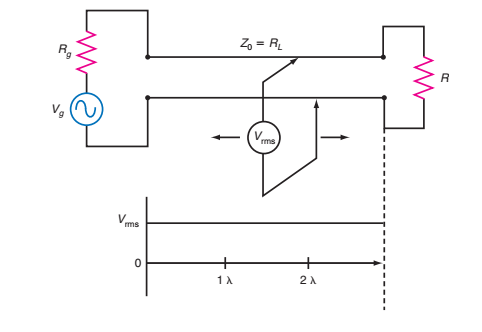
\includegraphics[width=.8\textwidth]{17.png}
\end{figure}

\indent 如果负载阻抗与线路特性阻抗不同,则不是所有传输的功率都被负载吸收。 未被负载吸收的功率被反射回源。 向负载下行的功率称为前向功率或入射功率; 未被负载吸收的功率称为反射功率。 实际上在一条线上的信号只是正向和反射信号的代数和。\\
\indent 反射的力量可以代表一个重大的损失。 如果一条线路的端到端损耗为3 dB,那么在信号到达发生器的时候,只会产生3 dB的相对衰减。 发生什么取决于发电机和线路的相对阻抗。 只有部分相关的能量在线路中消失。 在负载电阻阻抗与线路阻抗不匹配的情况下,反射功率足够高,实际上会对发射机或线路本身造成损害。\\

\subsection{短路线}
短路情况如图13-18所示。 传输线下面的图表显示了线路上每个点的电压和电流的曲线,这些电压和电流可以通过使用由电压表和电流表给出的值来产生。 正如在线路末端短路的情况下所期望的那样,当电流最大时电压为零。 所有的功率都反向回到发生器。 看图,你可以看到电压和电流变化根据信号波长分布。 正向和反向信号复合后的固定模式每隔半个波长重复一次。 发生器的电压和电流水平取决于信号波长和线路长度。\\
\indent 线路发电机端的相电压的相位取决于线路的长度。 如果这条线是四分之一波长的几倍,则反射波将与入射波同相,二者将相加,在发生器处产生一个信号,该信号是发生器电压的两倍。 如果线路长度是半个波长的几倍,则反射波与入射波的相位相差180°,二者将抵消,在发生器处产生一个零电压。 换句话说,反射波的影响可以模拟发电机的开路或短路。\\

\hrule
\medskip
\noindent\textbf{图13-18} 在短路传输线上驻波。\\
\begin{figure}[!h]
\centering
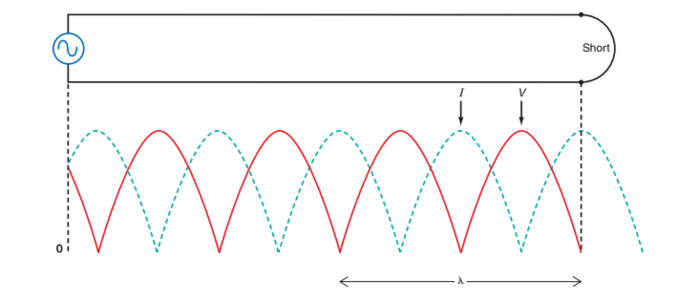
\includegraphics[width=.8\textwidth]{18.png}
\end{figure}

\subsection{开路线}
图13-19显示了开路线上的驻波。 在无限的阻抗负载下,当电流为零时,线路末端的电压最大。 所有的能量相互关联,建立起电压和电流驻波的固定模式。\\

\hrule
\medskip
\noindent\textbf{图13-19} 驻扎在开路传输线上。\\
\begin{figure}[!h]
\centering
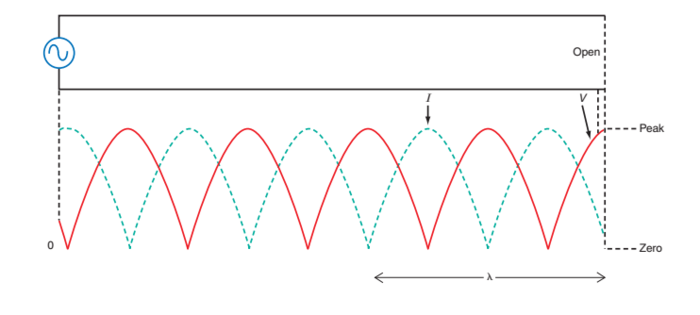
\includegraphics[width=.8\textwidth]{19.png}
\end{figure}

\subsection{不匹配(共振)线}
大多数情况下,线路不会以短路或开路形式终止。 相反,负载阻抗并不完全匹配传输线阻抗。 此外,负载(通常是天线)除了其电阻外,可能还会具有电感性或电容性的电抗元件。 在这些条件下,这条线被认为是共振的。 这种不匹配会产生驻波,但这些波的振幅比由短路或开路产生的驻波低。 这些驻波的分布如图13-20所示。 请注意,电压或电流永远不会变成零,就像开路或短路那样。\\

\bigskip
\hrule
\medskip
\noindent\textbf{图13-20} 传输线与负载不匹配,导致驻波。\\
\begin{figure}[!h]
\centering
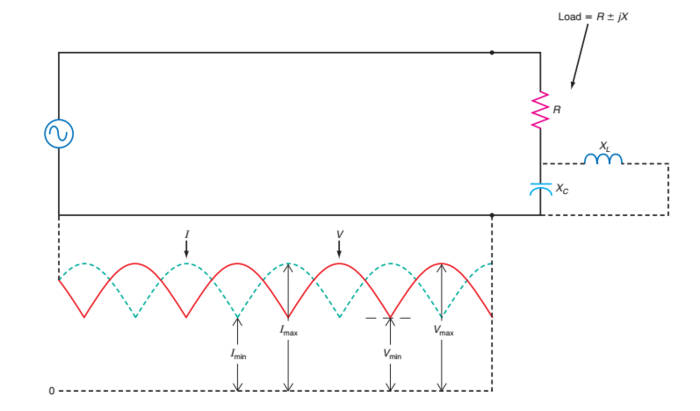
\includegraphics[width=.8\textwidth]{20.png}
\end{figure}

\subsection{计算驻波比}
传输线上驻波的大小取决于沿线的最大电流与最小电流的比值,或者最大电压与最小电压的比值。 这些比率被称为驻波比(SWR)。
$$SWR = \frac{I_max}{I_min} = \frac{V_max}{V_min}$$\\
\indent 在前面所述的短路和开路条件下,电流或电压最小值为零。 这产生了一个无限的SWR。 这意味着负载没有功率消耗; 所有的力量都体现出来了。\\
\indent 理想情况下,没有驻波。 电压和电流沿线是恒定的,所以没有最大值或最小值(或最大值和最小值相同)。 因此,SWR是1。\\
\indent 测量线路上的电压和电流的最大值和最小值在现实世界中是不实际的,因此已经设计了其他计算SWR的方法。 例如,如果传输线的阻抗和负载的实际阻抗已知,则可以计算SWR。 SWR是负载阻抗$Z_1$与特性阻抗$Z_0$的比值,反之亦然。\\
\indent If $Z_t$ > $Z_0$
$$SWR = \frac{Z_t}{Z_0}$$\\
\indent If $Z_0$ > $Z_t$
$$SWR = \frac{Z_0}{Z_t}$$\\
\indent 例如,如果将75 V天线负载连接到50 V传输线,则SWR为75/50 = 1.5。 由于驻波实际上是原始入射波加到相关波上的复合波,所以SWR也可以用这些波来定义。 相关电压波形$V_r$与入射电压波形$V_i$的比值称为相对系数
$$ \Gamma = \frac{V_r}{V_i}$$\\
\indent 反射系数提供沿线的电流和电压信息。 另外,$\Gamma$ = 反射功率/入射功率。
\indent 如果一条线路的特性阻抗被终止,那么没有相反的电压,所以$V_r = 0$和$\Gamma = 0$。如果线路开路或短路,则发生总体反向。 这意味着$V_r$和$V_i$是相同的,所以$\Gamma = 1$。实际的相对系数表示相对于入射电压的相对电压的百分比。 例如,如果$\Gamma$是0.5,则反射电压是入射电压的50%,并且反射功率是入射功率的百分之25[$\Gamma^{2} = (0.5)^{2} = 0.25$]。\\
\indent 如果负载不匹配,但也不是开路或短路,则线路将具有最小电压和最大电压,如前所述。 这些可以用来通过使用公式来获得反射系数
$$\Gamma = \frac{V_{max} - V_{min}}{V_{max} + V_{min}} = \frac{SWR - 1}{SWR + 1}$$\\
\indent SWR是根据方程从反射系数中获得的
$$SWR = \frac{1 + \Gamma}{1 - \Gamma} = \frac{1 + \sqrt{p_r/p_i}}{1 - \sqrt{p_r/p_i}}$$

\bigskip
\hrule
\medskip
\noindent\textbf 例13-5\\
\noindent RG-11 / U泡沫同轴电缆的最大电压驻波为52 V,最小电压为17 V。(a)SWR,(b)相关系数,以及(c)阻性负载的值。\\
\noindent a. $SWR = \frac{V_max}{V_min} = \frac{52}{17} = 3.05$\\
\noindent b. $\Gamma = \frac{V_max - V_min}{V_max = V_min} = \frac{52 - 17}{52 + 17} = \frac{35}{69}$
\smallskip
$\Gamma = 0.51$
or
\smallskip
$\Gamma = \frac{SWR - 1}{SWR + 1} = \frac{3.05 - 1}{3.05 + 1} = \frac{2.05}{4.05} = 0.51$\\
\noindent c. $SWR = 3.05$ \quad $Z_0 = 75 Ω$  $SWR = \frac{Z_l}{Z_0} = \frac{Z_0}{Z_l}$
\smallskip
$Z_l = Z_0(SWR) = 75(3.05) = 228.75 Ω$
\smallskip
or
\smallskip
$Z_l = \frac{Z_0}{SWR} = \frac{75}{3.05} = 24.59 Ω$\\



如果负载匹配线路阻抗,则$\Gamma = 0$.上述公式给出SWR为1,如预期。 负载开路或短路时,$\Gamma = 1$。这产生无穷大的SWR。\\
\indent 反射系数也可以由线路和负载阻抗确定:
$$\Gamma = \frac{Z_t - Z_0}{Z_t + Z_0}$$
对于75 V的天线负载和50 V的同轴电缆,反射系数为$\Gamma =(75 - 50)/(75 + 50)= 25/125 = 0.2$。\\
\indent SWR的重要性在于它给出了输电线路和发电机损失多少功率的相对指示。 这假定反射的功率都没有被发生器重新相关。 在典型的发射机中,一些功率被反射并再次发送到负载。\\
\indent 图13-21中的曲线显示了相对功率百分比与SWR之间的关系。 相对功率的百分比也用回损表示,并以瓦或分贝(dB)表示。 自然,当驻波比为1时,相对功率百分比为0.但是随着线路和负载失配的增加,相对功率增加。 当SWR为1.5时,反射功率百分比为4%。 这还不算太坏,因为96%的功率达到了负载。\\

\indent 如果给定SWR和入射功率$P_1$,则可以计算相关功率$P_r$。 由于$\Gamma^{2} = P_r / P_i$,所以$P_r = \Gamma^{2}P_i$。 知道了SWR,你可以计算$\Gamma$,然后用前面的方程求解。
$$\frac{P_r}{P_i} = \Gamma^{2} = (\frac{SWR - 1}{SWR + 1})^{2}$$
$$= (\frac{1.5 -1}{1.5 + 1})^{2}$$
$$= 0.2^{2}$$
$$= 0.04$$
$$\frac{P_r}{P_i} = 4\%$$
计算SWR的最好和最实用的方法之一是测量正向功率$P_f$和反向功率$P_r$,然后用公式
$$SWR = \frac{1 + \sqrt{P_r/P_i}}{1 - \sqrt{P_r/P_i}}$$
发明了几个好的电路来测量正向和反向功率。 而且,商业测试仪器也可以插入传输线并进行这些测量。 数据从前面板仪表或数字显示屏上读取。 然后将数据插入上面的公式中。 一些精密的测试仪器有一个内置的嵌入式计算机来自动计算并显示SWR值。\\

\hrule
\medskip
\noindent\textbf{图13-21} 对于不同的SWR值,在传输线上反射功率的百分比。\\
\begin{figure}[!h]
\centering
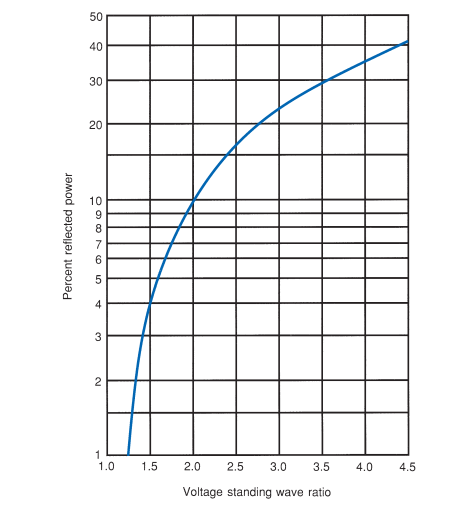
\includegraphics[width=.8\textwidth]{21.png}
\end{figure}

\indent 例如,假设您测量35 W的正向功率和7 W的反射功率。SWR是
$$SWR = \frac{1 + \sqrt{7/35}}{1 - \sqrt{7/35}} = \frac{1 + \sqrt{0.2}}{1 - \sqrt{0.2}}$$
$$SWR = \frac{1 + 0.4472}{1 - 0.4472} = \frac{1.4472}{0.5528}$$
$$SWR = 2.618$$
您将了解最常见的功率测量电路和设备在第22章。\\
\indent 对于2或更小的SWR值,相对功率小于10%,这意味着90%的负载。 对于大多数应用程序这是可以接受 对于高于2的SWR值,相对功率百分比急剧增加,必须采取措施降低SWR以防止潜在的损害。 如果SWR大于2,则一些固态系统会自动关闭。降低SWR的最常见方法是添加或包含π,L或T LC网络来抵消天线电抗和其他电阻元件,并产生一个阻抗匹配。还可以调整天线长度以改善阻抗匹配。\\

\bigskip
\hrule
\medskip
\noindent\textbf 例13-6\\
\noindent 例13-5中的线路输入是30W。输出功率是多少?(见图13-21;不考虑由于长度造成的衰减)。\\
\indent SWR为3.05的相对功率百分比约为25.62。\\
$$P_r = 0.2562(30 W) = 7.686 W$$
\noindent 或者,$$P_r = P_i (\frac{SWR - 1}{SWR + 1})^{2}$$\\
$$ =30(\frac{3.05 - 1}{3.05 + 1})^{2}$$
$$ = 7.686 W$$
$$ P_out = P-i - P_r = 30 - 7.686 = 22.314 W$$

\section{传输线作为电路元件}
与传输线一起工作时,通常必须避免由开路和短路负载产生的驻波条件。 然而,对于四分之一波长和二分之一波长的传输,这些开路和短路负载可以用作谐振电路或反应电路。\\

\subsection{谐振电路和反应元件}
考虑如图13-22所示的短路四分之一波长(λ/ 4)线。 在负载端,电压为零,电流最大。 但四分之一波长回到发生器,电压最大,电流为零。 对于发生器来说,该线路表现为开路,或至少是非常高的阻抗。 这里关键的一点是,这种情况只存在于一个频率上,频率恰好是四分之一波长的频率。 由于这种频率敏感性,线路起到LC调谐或谐振电路的作用,在这种情况下,它是一个并联谐振电路,因为它在参考频率处具有非常高的阻抗。\\


\hrule
\medskip
\noindent\textbf{图13-22} 短路的四分之一波长线用作并联谐振电路。\\
\begin{figure}[!h]
\centering
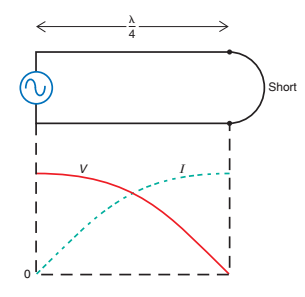
\includegraphics[width=.4\textwidth]{22.png}
\end{figure}

\hrule
\medskip
\noindent\textbf{图13-23} 短路的一半波长线用作串联谐振电路。\\
\begin{figure}[!h]
\centering
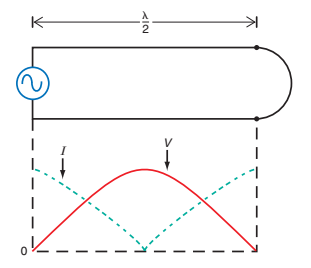
\includegraphics[width=.4\textwidth]{23.png}
\end{figure}


\indent 在短路的一半波长线上,驻波图如图13-23所示。 发生器看到与线末端相同的条件,即零电压和最大电流。 这表示一个短的,或者非常低的阻抗。 这种情况只有在发电机的频率恰好等于半波长的情况下才会发生。 在这种情况下,该线看起来像发电机的串联谐振电路。\\
\indent 如果在工作频率下,线路长度小于四分之一波长,则短路线看起来像是发电机的电感。 如果短路线在四分之一到二分之一波长之间,则看起来像发电机的电容器。 所有这些情况都以短路线的多个四分之一或二分之一波长重复。\\
\indent 如图13-24所示,用一条开放的线获得了类似的结果。 对于发生器来说,四分之一波长线看起来像一个串联谐振电路,而一个半波长线看起来像一个并联谐振电路,恰好与短路线相反。如果该线小于四分之一波长, 发生器看到一个电容。 如果线路在四分之一波长到二分之一波长之间,那么发生器就会看到一个电感。这些特性重复用于四分之一或二分之一波长倍数的线路。\\

\hrule
\medskip
\noindent\textbf{图13-24} 四分之一和二分之一波长的开路线看起来像发电机的谐振电路。\\
\begin{figure}[!h]
\centering
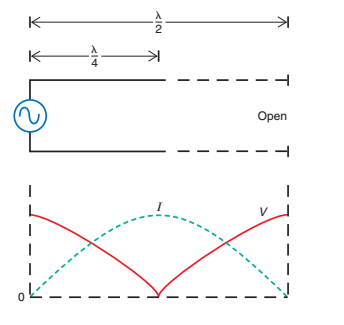
\includegraphics[width=.4\textwidth]{24.png}
\end{figure}

\indent 图13-25是长达一个波长的开路和短路线所表示的条件的总结。 横轴是波长的长度,垂直轴是线路的电抗,以欧姆为单位,以线路特性阻抗表示。 实线曲线为短线,虚线为开路线。\\

\hrule
\medskip
\noindent\textbf{图13-25} 短路和开路线路的阻抗和电抗变化的总结,长度可达一个波长。\\
\begin{figure}[!h]
\centering
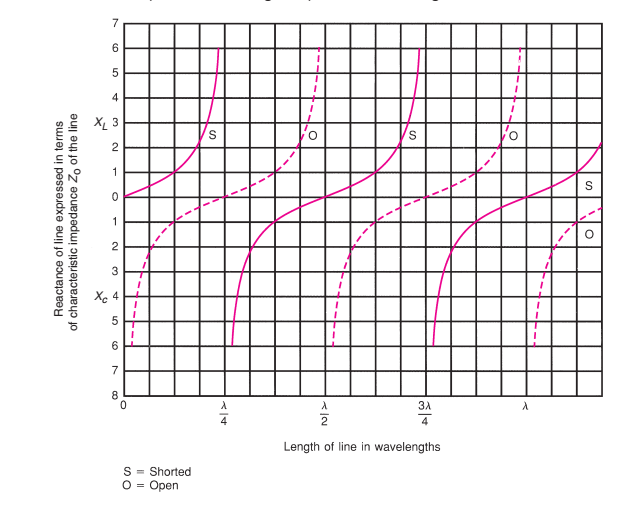
\includegraphics[width=.8\textwidth]{25.png}
\end{figure}

\indent 如果该线用作串联谐振电路,则其阻抗为零。 如果线路的长度足以构成并联谐振电路,则其阻抗接近于零。 如果线路是中间长度的话,它是被动的。 例如,考虑一个短的八分之一波长线。 水平分割表示十六分之一波长,所以其中两个表示八分之一波长。 假设该线路的特征阻抗为50 V。在左侧实线的八分之一波长点上的读数为1.这意味着该线路作为$1 × Z_0$的感抗,或者$1 × 50 = 50 Ω$。如图13-24中最左边的虚线所示,约三分之八波长的开放线具有相同的效果。\\
\indent 用同样的50Ω线路怎么能够产生150Ω的容抗? 首先,在图13-25的容性电抗标尺上找到150-Ω点。 由于150/50 = 3,150-Ω点在$X_C = 3$。接下来,从该点向右画一条直线,直到它与两条曲线相交。 然后从水平刻度读取波长。 50伏线路的电容电抗可以用稍长于1/32波长的开路线或比9/32波长稍长的短路线来实现。\\

\subsection{带状线和微带}
在低频率(低于大约300MHz)时,前面讨论的开路和短路线路的特征几乎没有意义。 在低频时,线路太长而不能用作电抗元件或滤波和调谐电路。然而,在UHF(300-3000MHz)和微波(1GHz及更高)频率下,半波长的长度是 小于1英尺; 电感和电容的值变得很小,很难用标准线圈和电容器来实现它们。 在印刷电路板(PCB)上构造的特殊传输线(称为微带或带状线)可以用作调谐电路,滤波器,移相器,电抗元件和阻抗匹配电路。\\
\indent 印刷电路板是由柏拉图或其他一些绝缘基底材料制成的绝缘基底,其一端或两端粘合铜,有时也粘合在若干层中。微波应用中某些印刷电路板的基底或陶瓷被用作基底。 在微波集成电路中,基体通常是氧化铝或蓝宝石。 铜被蚀刻掉形成晶体管,集成电路,电阻和其他组件的互连,从而消除了与导线的点对点连接。 二极管,晶体管和其他组件直接安装在PCB上,并直接连接到形成的微带或带状线。\\

\bigskip
\hrule
\medskip
\noindent\textbf{图13-26} 微带(a)不平衡。 (b)平衡。\\
\begin{figure}[!h]
\centering
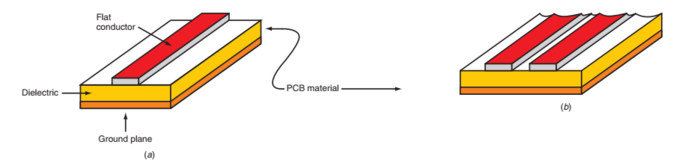
\includegraphics[width=.8\textwidth]{26.png}
\end{figure}

\bigskip
\bigskip
\bigskip
\hrule
\medskip
\noindent\textbf{图13-27} 计算特性阻抗的尺寸。\\
\begin{figure}[!h]
\centering
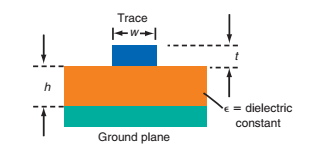
\includegraphics[width=.6\textwidth]{27.png}
\end{figure}


\hrule
\medskip
\noindent\textbf{图13-28} 带状线。\\
\begin{figure}[!h]
\centering
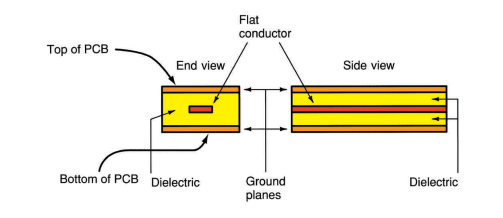
\includegraphics[width=.8\textwidth]{28.png}
\end{figure}

\subsubsection{微带}
微带线是由绝缘介质与大的导电接地层分开的扁平导体[图13-26的(a)]。 微带通常是四分之一或半波长。 地平面是常见的电路。 这种类型的微带线相当于不平衡的线路。 空行通常优先于空行。 微带也可以制成双线平衡版本[图13-26(B)]。\\
\indent 与任何传输线一样,微带的特性阻抗取决于其物理特性。 可以用公式来计算
$$Z = \frac{87}{\sqrt{ε+ 1.41}}ln\frac{5.98h}{0.8w + t}$$
其中Z =特性阻抗,ε=介电常数,w =铜线的宽度,t =铜线的厚度,h =电介质的迹线与接地平面(电介质厚度)之间的距离。
可以使用任何度量单位(例如,英寸或毫米),只要所有尺寸都在相同的单位中即可。(见图13-27)流行的FR-4玻璃纤维PC板材料的介电常数为4.5。ε的值是3。\\
\indent 尺寸为h = 0.0625in,w = 0.1in,t = 0.003in和ε= 4.5的微带特征阻抗为
$$Z = \frac{87}{\sqrt{4.5+ 1.41}}ln\frac{5.98(.0625)}{0.8(0.1) + 0.003}$$
$$=35.8ln4.5 = 35.8(1.5)$$
$$Z = 53.9Ω$$\\
\subsubsection{带状线}
带状线是夹在两个地平面之间的导体(图13-28)。 比微带制作更难; 但是,它不像微带那样辐射。 辐射会造成损失。 长度是所需工作频率的四分之一或二分之一波长,短路线比开路线更常用。\\
\indent 带状线的特征阻抗由公式给出
$$Z = \frac{60}{ε}ln\frac{4d}{0.67πw(0.8 + t/h)}$$
图13-29显示了进行计算所需的尺寸。\\
\indent 即使是较小的微带线和带状线也可以通过使用单片,薄膜和混合IC技术来制造。 当这些与二极管,晶体管和其他组件结合时,形成微波集成电路(MIC)。\\

\section{史密斯图}
设计和分析传输线路所需的数学工作是复杂的,无论该线路是将收发器连接到天线还是用作滤波器或阻抗匹配网络的物理电缆。 这是因为所涉及的阻抗是复杂的,涉及电阻和电抗元件。 阻抗采用熟悉的矩形形式R ± jX。 像这样的复数的计算是漫长而费时的。\\
\indent 对于你在这里看到的每一个天线,都有一条传输线。 同轴电缆是最常见的,但波导用于微波。此外,许多计算涉及三角关系。 尽管没有单独的计算是很困难的,但是计算的绝对数量可能会导致错误。\\
\indent 在二十世纪三十年代,一位聪明的工程师决定做一些事情来减少传输线计算错误的可能性。 工程师的名字是Philip H. Smith,1939年1月,他出版了史密斯圆图,这是一个复杂的图形,可以对传输线计算进行可视化解决方案。\\
\indent 当然,今天,由于电子计算选择的广泛可用性,传输线计算的数学不成问题。 传输线方程可以很容易地编程到科学和工程计算器中,以获得快速,简单的解决方案。 个人电脑提供了一种理想的方式来进行这些计算,可以使用特殊的数学软件包,也可以使用BASIC,Fortran,C或其他语言编写特定的程序。 如果需要的话,现在常用于工程和科学计算的数学软件包也提供图形输出。\\
\indent 尽管今天所有的计算选项都可用,但史密斯圆图仍在使用。 其独特的格式为查看和解决输电线路及相关问题提供了或多或少的标准化方法。 此外,等式的图形表示传达的信息比通过对方程的简单检查所获得的信息更多。由于这些原因,期望熟悉史密斯圆图。\\
\indent 图13-30是史密斯圆图。 通过在第三个圆上绘制两组正交(直角)圆来创建该强加图。 史密斯圆图纸可以从最初的出版商,模拟仪器公司和美国无线电中继联盟获得。 史密斯图表图纸也可在一些大学和大学书店。\\
\indent 创建史密斯圆图的第一步是沿水平线绘制一组偏心圆,如图13-31所示。 横轴是纯电阻或零电位线。 线的最左端的点表示零电阻,而最右边的点表示无限电阻。 阻力圆线集中在这条纯阻力线上并穿过这条阻力线。 在无穷大的阻力点上,所有圆都相切,所有圆的中心落在阻力线上。\\
\indent 每个圆圈代表一些固定电阻值的所有点。 外圆上的任何一点代表0Ω的电阻。其他圆圈有其他电阻值。 R = 1圆通过阻力线的正确中心,被称为主中心。 纯电阻值和传输线特性阻抗值绘制在这条线上。\\
\indent 目前使用的最常见的传输线阻抗是50V。因此,大部分阻抗和电抗都在50V范围内。 那么50伏的值位于图表的主要中心是很方便的。 这意味着R = 1圆上的所有点代表50Ω,R = 0.5圆上的所有点代表25Ω,R = 2圆上的所有点代表100 Ω,依此类推。\\
\indent 史密斯圆图是所谓的归一化形式,R = 1在主要中心。用户通过为主要中心分配不同的值来为特定应用定制史密斯圆图。\\
\indent 史密斯圆图的其余部分通过添加电抗圆来完成,如图13-32所示。 像电阻圆一样,这些都是古怪的,所有的圆都在无限的阻力点上相遇。 每个圆圈表示一个恒定的电抗点,感应电抗圆圈在顶部,电容电抗在圆圈底部。注意图表上的电抗圆是不完整的。 图表中只包含R = 0行内的那些圆圈部分。与电阻圆一样,反应圆也以标准化形式呈现。比较图13-31和13-32到图13-30中的完整史密斯圆图,然后再继续。\\

\subsection{绘制和读取阻抗值}
图13-33中的史密斯圆图显示了绘制的阻抗值的几个例子:
$$Z_1 = 1.5 + j0.5$$
$$Z_2 = 5 - j1.6$$
$$Z_3 = 0.2 + j3$$
$$Z_4 = 0.4 - j0.36$$
找到史密斯圆图上的每个点,并确保您了解每个点是如何获得的。\\
\indent 图13-33中绘制的阻抗值是标准化值。 将史密斯圆图放大到特定的阻抗范围需要将这些值乘以某个公因子。 例如,许多史密斯圆图在主要中心以50伏绘制。 上面列出的50V的中心值的阻抗如下:
$$Z_1 = 75 + j25$$
$$Z_2 = 250 - j80$$
$$Z_3 = 25 + j150$$
$$Z_4 = 20 - j18$$
\indent 为了解决实际阻抗值的问题,将阻抗值和无功值除以一个等于素数中心电阻值的因子,将其归为归一化形式。 然后绘制数字。\\
\indent 当您读取归一化史密斯圆图的数值时,将其转换为标准阻抗形式,方法是将电阻和电抗乘以一个等于素数中心电阻的因数。\\

\subsection{波长标尺}
图13-30中史密斯圆图的外周上的三个刻度是朝向发生器的波长,朝向负载的波长以及以度数表示的相对角度。 标记为“朝向发电机”的刻度从零电阻和零电抗线开始顺时针移动到无限电阻位置。圆形旋转的一半是90°,在史密斯圆图上, 四分之一波长 一个完整的旋转是半波长。 沿着一条线分布的电压和电流的传输线模式每半个波长重复一次。\\
\indent 标有“朝向负载”的刻度也从零电阻零电抗点开始,沿逆时针方向进行一个完整的旋转或半个波长。 无限电阻点是四分之一波长标记。\\
\indent 相对系数(相对电压与入射电压的比值)的范围为0到1,但也可以表示为从0º到360º,从0º到正180º,或从0º到 减去180º。 零标记位于电阻线右侧的无限电阻点上。\\

\subsection{SWR圈}
史密斯圆图上绘制的传输线的SWR是一个圆圈。 如果负载是电阻性的并且与线路的特性阻抗相匹配,则驻波比为1。在史密斯圆图的主中心将其绘制为单个点。 线路的阻抗为50Ω时的阻抗或任何其他标准值。 但是,如果负载不能完全匹配到阻抗,驻波就会存在。 在这种情况下的SWR由以中心为主中心的圆表示。\\
\indent 为了绘制一个SWR圆,首先使用之前给出的公式计算SWR。 对于这个例子,假设SWR为2.从素数中心开始,在阻力线上向右移动,直到遇到值2。 然后,使用绘图指南针,将该点放置在中心,并通过素数中心右侧的2标记绘制一个圆圈。 圆也应该通过总理中心左边的0.5标记。 图13-33中绘制的红色圆圈表示沿着不匹配或谐振传输线的阻抗变化曲线。 电压和电流驻波的变化意味着沿线的阻抗存在连续的变化。 换句话说,不匹配线路上一个点的阻抗与线路上所有其他点的阻抗不同。 所有阻抗值出现在SWR圆上。\\
\indent SWR圆也可以用来确定沿线的最大和最小电压点。 例如,SWR圆与素数中心右侧的电阻线相交的点指示来自负载的波长驻波的最大或峰值电压点。 这也是线路上的最大阻抗点。 SWR圆通过质心左侧的电阻线的点表示最小电压和阻抗点。\\
\indent 在史密斯圆图底部印刷的线性刻度用于计算SWR,dB损耗和相关系数。 例如,要使用线性SWR比例,只需绘制一条与SWR圆相切的直线,并垂直于史密斯圆图左侧的阻力线。 使线条足够长,以使其与图表底部的SWR比例相交。 这已经在图13-33中完成了。 请注意,值为2的SWR圆可以从线性SWR刻度中读取。\\

\subsection{使用史密斯圆图:例子}
如上所述,当负载与特定应用中的特性阻抗不匹配时,线路的长度变成发电机看到的总阻抗的一部分。 史密斯圆图提供了一种方法来找到这个阻抗。 一旦阻抗已知,可以添加一个阻抗匹配电路来补偿这些条件,使线路l和SWR尽可能接近1。\\
\subsubsection{图13-34的实例1}
24英尺长的RG-58A / U同轴电缆的工作频率为140 MHz。 负载是电阻性的,电阻为93 V。变送器看到的阻抗是多少?\\
\indent 第一步是找到由24英尺电缆表示的波长数量。 140-MHz信号的波长为
$$λ = \frac{948}{f} = \frac{948}{140} = 7.02ft$$
请记住,由于电缆中的RF信号减速,同轴电缆的速度因子小于1。 RG-58A / U的速度系数为0.66。 因此,一个140 MHz的波长是
$$λ = 7.02 × 0.66 = 4.64ft$$
由24英尺电缆表示的波长数目是24 / 4.64 = 5.17λ。\\
\indent 如前所述,沿着一条线的阻抗变化重复每半个波长,因此每个全波长; 因此为了计算,我们只需要上述数值的0.17λ。\\
\indent 接下来,我们将史密斯圆图归一化为53.5Ω的同轴电缆的特征阻抗。主中心的值为53.5Ω。然后计算SWR:
$$SWR = \frac{Z_1}{Z_0} = \frac{93}{53.5} = 1.74$$
这个SWR现在被绘制在史密斯圆图上。 参见图13-35,其中点X表示93Ω的电阻负载。\\
\indent 为了找到同轴电缆发射端的阻抗,我们沿5.17的λ线从负载回到发射器或发生器。 请记住,围绕史密斯圆图的一个完整的旋转是半个波长,因为这些值重复每半个波长。 从X点开始,然后顺时针方向(朝向发电机)围绕SWR圆周运动10次,这代表5λ。 这使你回到X点。\\
\indent 继续顺时针旋转0.17λ,停在那里,并在SWR圆上标记该点。 画一条从素数中心到代表0.17λ的位置的直线。 点X右边的标记是0.25-λ标记。 你需要从0.17λ,或0.25 + 0.17 = 0.42。 在Y的圆圈下部的0.42标记处停下。从那里画一条线到素数中心。 再参考图13-35。\\
\indent 线切割SWR圆的点是发电机看到的阻抗。 从图表中读取数值,你有R ≈0.68和$X_C$ ≈0.35。 由于该点位于图的下半部分,所以电抗是电容性的。 因此此时的阻抗为0.68 - j0.35。\\
\indent 为了找到实际值,通过乘以主要中心的阻抗来从归一化值转换成53.5:
$$Z = 53.5(0.68 - j0.35) = 36.4 - j18.725 Ω$$\\
\indent 发射器看到的是一个36.4V电阻串联一个电抗为18.725V的电容。等效电容值是[使用$X_C = 1/(2πfC)$或$C = 1y(2πfX_C)$]
$$C = \frac{1}{6.28(140×10^{6})(18.725)} = 60.74 pF$$
等效电路如图13-34(b)所示。\\

\subsubsection{图13-36的实例2}
天线与示例1中所述的24英尺53.5-Ω RG-58A / U线相连。负载为40 + j30 Ω.发射器看到什么阻抗?\\
\indent 主要中心是53.5 Ω,像以前一样。 绘制图表上的负载阻抗之前,必须将其归一化为53.5:
$$Z_l = \frac{40 + j30}{53.5} = 0.75 + j0.56$$\\
\indent 这个值的图如图13-36所示。 请记住所有的阻抗落在SWR圆上。 您可以简单地通过将指南针放置在负载阻抗点的半径上并旋转360°的素数中心来绘制SWR圆。\\
\indent 通过垂直于阻力轴的直线延伸到SWR线,从图表底部的图表中获得SWR。 SWR约为2; 1。\\
\indent 下一步是通过绘制的负载阻抗从素数中心画出一条线,使其与曲线周边的波长刻度相交。 再次参考图13-36。 因为我们的参考起点是负载阻抗,所以我们使用“朝向发生器”的比例来确定线路输入端的阻抗。 在点X是0.116的波长值。\\
\indent 现在,由于发生器距离负载为5.17λ,并且由于读数每半个波长重复一次,所以您朝顺时针方向0.17λ移动发生器:0.116和0.17 = 0.286。 这一点在图13-36中标记为Y。\\
从Y点到素数中心绘制一条线。 它与SWR圆相交的点表示发生器看到的阻抗。 归一化的值是1.75 - j0.55。 纠正这个53.5 Ω总理中心,我们得到
$$Z = 53.5(1.75 - j0.55) = 93.6 - j29.4 Ω$$
这是发电机看到的阻抗。\\

\subsubsection{图13-37的实例3}
在很多情况下,天线或其他负载阻抗是未知的。 如果线路不匹配,线路会修改阻抗,使发射机看到不同的阻抗。 找到总体阻抗以及天线或其他负载阻抗的一种方法是使用阻抗桥来测量发射机端的负载和传输线的组合阻抗。 那么史密斯圆图可以用来找到单个阻抗值。\\
\indent 具有75V的特征阻抗和0.8的速度因子的50英尺RG-11 / U泡沫介电同轴电缆的工作频率为72MHz。 负载是实际阻抗未知的天线。 电缆发射端的测量结果为82 + j43的复数阻抗。 什么是天线的阻抗?\\
\indent 在72 MHz的一个波长是984/72 =在72 MHz的一个波长是984y72 5 13.67 ft。考虑速度因素的收益率 13.67 ft。考虑速度因素的收益率
$$λ = 13.67 × 0.8 = 10.93 ft$$
50英尺长的电缆的长度为50 / 10.93 = 4.57。 如前所述,这是实际使用的0.57λ值。\\
\indent 首先,测量的阻抗被标准化并绘制。 主要中心是75 V.图13-37 Z =(82 + j43)/75 = 1.09 + j0.52绘制在史密斯圆图上。 这个SWR圆是通过这个点从中心点绘制的。 然后从圆圈画出一条切线到底部的线性SWR图表。 SWR是1.67。\\
\indent 接下来,从素数中心到归一化阻抗点并通过曲线图周边的波长图画出一条线。 它与X点处的“朝向负载”尺度相交,即0.346λ。 参考图。\\
\indent 在发电机端看到的阻抗是标准值,所以有必要沿逆时针方向绕着负载移动到负载阻抗。 我们移动的距离等于电缆的长度,即4.57λ。 从X点开始的9个完整的旋转表示4.5λ,这使我们回到X点。然后,我们再旋转0.07λ,逆时针旋转完成长度。 这使得我们在0.346 + 0.07 = 0.416λ点,在图13-37中被指定为点Y. 然后我们画一条从Y到主要中心的线。 这条线与SWR圆相交的点是实际的天线阻抗。 归一化的值是0.72 + j0.33。 乘以75得到天线阻抗的实际值:
$$Z = 75(0.72 + j0.33) = 54 + j24.75 Ω$$\\

\section{本章回顾}
 在线活动\\
 同轴电缆变化\\
\begin{multicols}{2}
\noindent\textbf{目的}:检查几种不同类型的同轴电缆。\\
 \textbf{步骤}:\\
 1. 使用标准的互联网搜索技术,寻找信息来回答以下问题。 搜索“同轴电缆制造商”或“同轴电缆类型”或类似术语。\\
 \textbf{问题}:\\
 1.最常见的同轴电缆特性阻抗是多少?\\
 2.什么是刚性同轴电缆,它在哪里使用?\\
 3.命名刚性同轴电缆的优点。\\
 4.你能找到的最高频率的同轴电缆是什么? 什么是在那个频率上的衰减?\\
 5.列出一个没有列出的同轴类型的同轴连接器\\
这本教科书。\\
\end{multicols}


\textbf{题目}\\
\begin{multicols}{2}
 \noindent 1.命名两种基本类型的传输线。哪个更广泛使用?\\
 2.传输线的两根导线之一接地的名称是什么?\\
 3.命名一种流行的平衡线。\\
 4.信号在一个周期内行进的距离是多少?\\
 5.命名用于同轴电缆的普遍的UHF连接器。\\
 6.测试设备和局域网中常用的同轴电缆连接器是什么?\\
 7.什么是UHF和微波应用的最佳同轴电缆连接器?\\
 8.什么类型的同轴连接器被广泛用于有线电视和录像机连接。\\
  9.描述传输线的等效电路。\\
 10.什么决定了传输线的特性阻抗?\\
 11.特性阻抗的另一个名称是什么?\\
 12.确定电缆长度的速度因子的重要性是什么?\\
 13.同轴电缆的截止频率如何随其长度而变化?\\
 14.描述适当匹配的传输线上的电流和电压的模式。\\
 15.描述如果传输线没有以其特性阻抗终止会发生什么。\\
 16.当负载和传输线阻抗不匹配时,对传输功率有什么影响?\\
 17.在哪两种情况下,所有事件的发生都会反映出来?\\
 18.传输线上的相对电压与入射电压之比是多少?\\
 19.你称之为不匹配的传输线?\\
 20.匹配传输线的长度如何影响SWR?\\
  21.说明用传输线实现串联谐振电路的两种方法。\\
 22.在工作频率下,小于λ/ 4或在λ/ 4和λ/ 2之间的传输线如何工作?\\
 23.史密斯圆图周围的一个完整的革命代表了多少个波长?\\
\end{multicols}

\textbf{问题}\\
\begin{multicols}{2}
 \noindent 1.计算频率为350 MHz的以米为单位的波长。 ◆\\
 2. 3.5倍长的线代表半波长的频率是多少?\\
 3.同轴电缆的电容为30 pF / ft,电感为78 nH / ft。什么是特征阻抗?\\
  4.同轴电缆的电容为17 pF / ft。特性阻抗是75 V.每英尺的等效电感是多少?\\
 5.介电常数为2.5的同轴电缆的速度系数是多少? ◆\\
 6.制造商的数据表指出,特定同轴电缆的速度系数是0.7。介电常数是多少?\\
 7.确定频率为49 MHz的速度因子为0.8的四分之一波长同轴电缆的长度(英尺)。 ◆\\
 8.使用Prob中给出的规格,同轴电缆引入的时间延迟是多少? 7如果长度是65英尺?\\
  9.介电常数为0.7的同轴电缆120英尺的时间延迟是多少? ◆\\
 10.同轴电缆引入多少相移15英尺长到10MHz的正弦波信号?介电常数是2.9。\\
 11.在100 MHz时,350 ft的RG-11 U同轴电缆的衰减是多少?\\
 12. 928 MHz的9913型同轴电缆的270 ft的近似衰减是多少?\\
 13.发射机具有3W的输出功率,通过20英尺长的RG-58A / U电缆馈送到天线。多少功率到达天线?\\
 14.从发电机到52V负载的最佳功率传输应该是什么样的传输线阻抗?\\
 15. 52 V同轴电缆具有36 V天线负载。什么是SWR?\\
 16.如果Prob中电缆的负载和线路阻抗。 15匹配,什么是SWR?\\
 17.传输线上的最大电压为170 V,最小电压为80 V.计算SWR和反射系数。\\
 18.传输线的相对系数是0.75。什么是SWR?\\
 19.开路或短路传输线的反射系数和SWR是多少?\\
 20.传输线的SWR为​​1.65。施加到线路上的功率是50W。反射功率的量是多少?\\
 21.插入传输线的功率表读取1150W的正向功率和50W的相对功率。什么是SWR?\\
 22.如果线路上的电压变化定期变为零,那么传输线上的负载阻抗值是多少?\\
 23.一根明线传输线6在多长时间内作为一个并联谐振电路? (电介质是空气。)\\
 24.同轴电缆的速度系数为0.68。这条电缆的波长在133 MHz处有多长时间?\\
 25.计算尺寸为h 5 0.05 in,w = 0.125 in,t = 0.002 in的微带线的阻抗。介电常数为4.5。\\
 26. Prob中微带四分之一波长的长度是多少? 25在915 MHz的频率?\\
 以标准化的形式绘出史密斯圆图上的以下阻抗:$Z_1 = 80 + j25$和$Z_2 = 35 - j98$,假设中心值为52 V。\\
 28.在史密斯圆图上的同轴线上绘制负载阻抗104 - j58。假设一个特征阻抗值为75 V.然后我发现SWR。\\
 29.如果工作频率为230 MHz,Prob电缆长度为30 ft。 28,如果速度因子是0.66,发电机的阻抗是多少?使用史密斯圆图并显示所有工作。\\
 30.史密斯圆图上的SWR圆是什么样的,如果一个52V负载连接到一个52V同轴电缆上?\\
  ◆选择问题的答案按照章节。22。\\
\end{multicols}

\textbf{批判性思维}\\
\begin{multicols}{2}
\noindent 1.如果线路短路或开路,请描述传输线路工作频率,工作频率为四分之一或二分之一波长。如何使用这样的线?\\
 2.在印刷电路板上实现传输线路的频率是多少?\\
 3.比较微带线和带状线的特性,哪个更好?为什么?\\
 4.阻抗为50 V的22英尺同轴电缆的速度系数为0.78。工作频率是400 MHz。天线负载阻抗与电缆发电机端测得的电缆阻抗相结合为74 +j66。什么是史密斯圆图上确定的天线阻抗?什么是SWR?\\
 5.假设在200英尺长的RG-58A / U同轴电缆上施加10 MHz的方波。它被正确地终止。在负载下描述信号,并解释信号为什么会出现。 (见图13-13)\\
 6.解释如何使用同轴传输线(RG-59 / U)作为滤波器来消除接收器输入端的干扰。假设频率为102.3 MHz。设计过滤器并计算大小。\\
\end{multicols}

\end{document}
\endinput
%%
%% End of file `husttrans-example.tex'.
